\chapter{The Transcorrelated Method for Multireference Problems}
\label{chap:binding}

This chapter is based in large part on the following upcoming publication:\\
\fullcite{haupt_sizeconsistent}

Images have been reused from this paper (with permission).

\section{Introduction}

In this chapter, we apply the new framework for the transcorrated method described in chapter \ref{chap:opt} to problems of multireference character and find these methods may yield unphysical results. We propose an updated workflow wherein we use conventional post-Hartree-Fock methods as input to Jastrow factor optimisation for TC-FCIQMC. Calculations suggest size-consistent results and rapid basis set convergence compared to conventional methods, with the binding curve of N$_2$ at \avtz being within chemical accuracy of experiment.

\section{Motivation}

A popular ``stress test'' for quantum chemistry methods is the binding curve of N$_2$. Highly accurate experimental results\supercite{leroyAccurate2006} exist to recreate the curve, allowing for a useful benchmark. At equilibrium, this system is essentially single reference in character, but as the bond is stretched, the system becomes strongly multireference, making it particularly challenging for many methods. As an example, we might consider standard \gls{CCSD}, which is a single-reference method, compared to FCIQMC which (within stochastic error) is exact.\footnote{We do not necessarily need an exact method to resolve this issue. Indeed, coupled cluster may be extended to be multireference, in which case it describes the N$_2$ binding curve very well.\supercite{lyakhMultireference2012}} Figure \ref{fig:ccsd-vs-fciqmc-n2} shows the binding curve of N$_2$ with CCSD compared to FCIQMC, using \vdz. We see that CCSD is not stable at large bond lengths.

\begin{figure}[htbp]
    \centering
    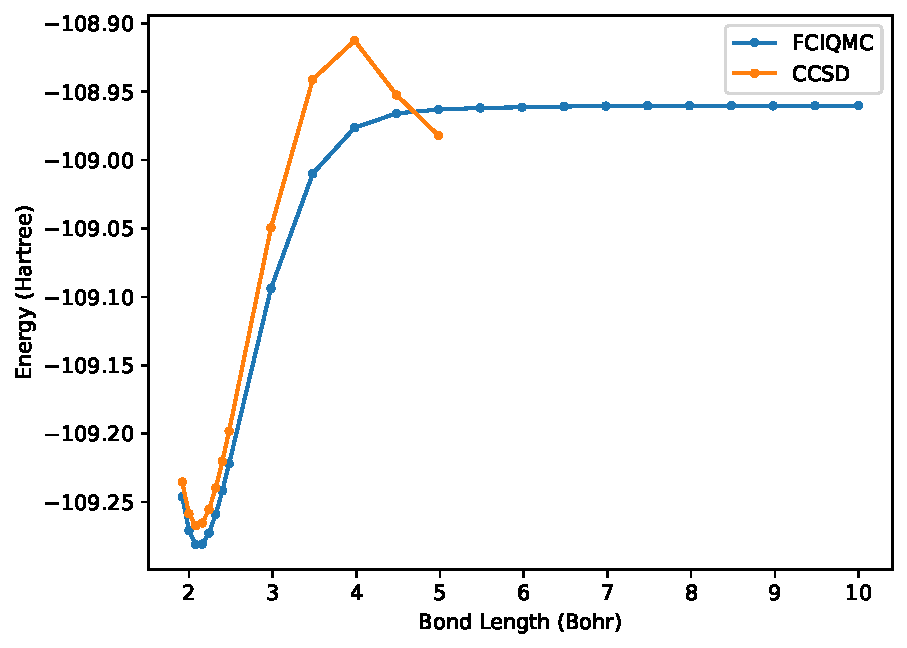
\includegraphics[width=0.9\textwidth]{figures/binding/N2_vdz_nontc}
    \caption{The binding curve for N$_2$ with the \vdz basis set. CCSD starts to decrease near 4 Bohr, which is unphysical, whereas FCIQMC provides a more accurate curve. This is because CCSD is a single-reference method, whereas FCIQMC is exact (within stochastic error). FCIQMC was done with 30 million walkers and HF-projected energy. CCSD did not converge at bond lengths larger than those shown.}
    \label{fig:ccsd-vs-fciqmc-n2}
\end{figure}

To see how well TC fares against such problems, consider the methodology outlined in chapter \ref{chap:opt}. We again use the same Jastrow factor as in equation \ref{eq:jastrow},
\begin{equation}
    \label{eq:jastrow-again}
    J = \sum_{i<j}^Nv(r_{ij}) + \sum_i^N\sum_I^{N_A}\chi(r_{iI}) + \sum_{i<j}^N\sum_I^{N_A}f(r_{ij}, r_{iI}, r_{jI}),
\end{equation}
with
\begin{equation}
    \label{eq:dtn-jastrow-ee-2}
    v(r_{ij})    = t(r_{ij},L_v)
                    \sum_{k} a_k r_{ij}^k ,
\end{equation}
\begin{equation}
    \label{eq:dtn-jastrow-en-2}
    \chi(r_{iI}) = t(r_{iI},L_\chi)
    \sum_{k} b_k r_{iI}^k ,
\end{equation}
\begin{equation}
    \label{eq:dtn-jastrow-een-2}
    f(r_{ij}, r_{i}, r_{j}) = t(r_{iI},L_f) t(r_{jI},L_f)
    \sum_{k,l,m} c_{klm}
    r_{ij}^k r_{iI}^l r_{jI}^m ,
\end{equation}
and the same cutoff functions $t(r,L) = (1-r/L)^3
\Theta(r-L)$. We also use the same objective function,
\begin{equation}
    \label{eq:varref-hf}
    \sigma_\mathrm{ref}^2 = \sum_{I\neq \mathrm{HF}}|\bra{D_I}\htc\ket{D_\mathrm{HF}}|^2,
\end{equation}
Using this workflow with the xTC approximation, we calculate points along the binding curve of N$_2$ with the \avtz basis set, and find a unphysical ``dip'', as shown in figure \ref{fig:binding-dip}, similar to what CCSD exhibits in figure \ref{fig:ccsd-vs-fciqmc-n2}, albeit much more subtle.

\begin{figure}[htbp]
    \centering
    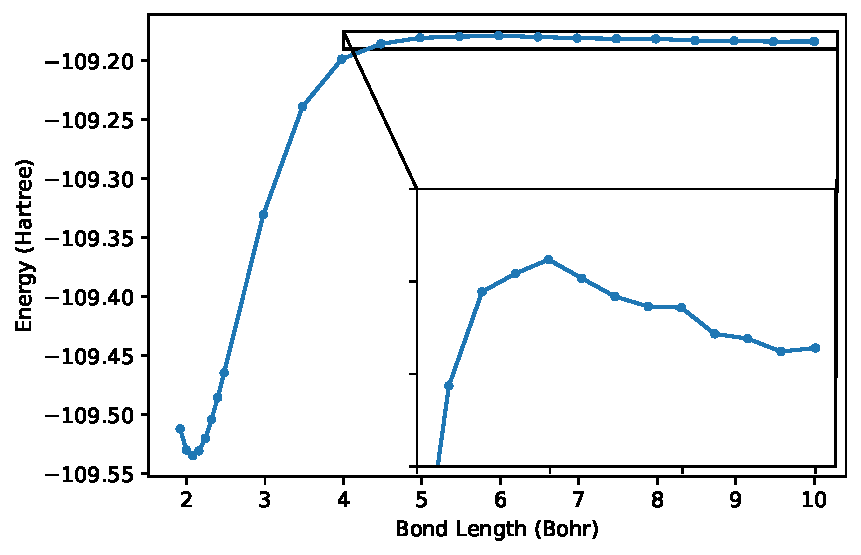
\includegraphics[width=0.8\textwidth]{figures/binding/inset_nontcfciqmc}
    \caption{The xTC-FCIQMC binding curve for N$_2$ with the \avtz basis set. While much smaller than that in figure \ref{fig:ccsd-vs-fciqmc-n2}, a unphysical dip is still present. This is apparent when zooming in on the curve, as shown in the inset.}
    \label{fig:binding-dip}
\end{figure}

This result has been verified for a few points with full TC (that is, with no approximations), which rules out xTC as the issue. Since the post-Hartree-Fock treatment was essentially at the FCI level, this implies that there is something wrong with the calculation of the Jastrow factors themselves. That is, our Hamiltonian is already ``corrupted'' before we even start the post-HF calculation.


\section{Resolving the Problem}

Based on the discussion in the previous section, it is likely that the transcorrelated workflow suffers from a single-reference bias. Indeed, the clear culprit is the Slater-Jastrow ansatz
\begin{equation}
    \label{eq:slater-jastrow-unichap}
    \Psi_\mathrm{SJ} = \e^J\Phi_\mathrm{HF},
\end{equation}
which affects the Jastrow optimisation and in turn the TC Hamiltonian $\htc = e^{-J}\hat H\e^J$.

We modify equation \ref{eq:slater-jastrow-unichap} to optimise for a multireference expansion,
\begin{equation}
    \label{eq:general-slater-jastrow}
    \Psi = \e^J\Phi_0
\end{equation}
where $\ket{\Phi_0}=\sum_I\ket{D_I}$. In practice, this modification results in two key changes in the workflow:
\begin{itemize}
    \item The objective function used during the VMC optimisation, equation \ref{eq:varref-hf}, needs to reflect the multireference ansatz. In particular, it will need to be changed to
    \begin{equation}
        \label{eq:varref-md}
        \sigma_\mathrm{ref}^2 = \sum_{I}|\bra{D_I}\htc\ket{\Phi_0} - \braket{D_I}{\Phi_0}\bra{\Phi_0}\htc\ket{\Phi_0}|^2,
    \end{equation}
    which is evaluated in VMC by sampling
    \begin{equation}
        S_\mathrm{ref}^2 =
          \frac 1 {n_\mathrm{opt}-1}
          \sum_{n=1}^{n_\mathrm{opt}}
            \left| \frac {\hat H({\bm R}_n) \Psi({\bm R}_n)}
                         {\Psi({\bm R}_n)} - {\bar E}_\mathrm{ref}
            \right|^2.
    \end{equation}
    \item The \gls{1RDM}, which is used in xTC during integration, must reflect this change as well. In particular, $\gamma_{p\dots}^{q\dots}=\bra{\Phi_0} a_{p\dots}^{q\dots}\ket{\Phi_0}$ in the equations in section \ref{sec:xtc}.
\end{itemize}

\subsection{Size Consistency}

One possible concern when studying problems like dissociation is that the method be size consistent. It is worth noting that one of the earliest Jastrow factors used for TC\supercite{boysCalculation1969} as well as in more recent work\supercite{cohenSimilarity2019} is given by
\begin{equation}
\label{eq:boyshandyjastrow}
J = \sum_{i<j} u(\bm r_i, \bm r_j)
\end{equation}
where
\begin{equation}
u(\bm r_i, \bm r_j) = \sum_{l,m,n}^{m+n+o\leq 6} c_{lmn}(\bar r_{iM}^m\bar r_{jN}^n+\bar r_{jM}^m\bar r_{iN}^n)\bar r_{ij}^l
\end{equation}
and $\bar r = r/(1+r)$.
However, notice that for $l=0$ and $n,m>0$, we can have non-vanishing gradients of $u$ for arbitrary distances between $N$ and $M$, and hence for systems $A$ and $B$ arbitrarily far apart we do not necessarily have
\begin{equation}
\label{eq:size-consistency}
e^{J_{A+B}}\ket{\Phi_{A+B}} = e^{J_0}(e^{J_{A}}\ket{\Phi_{A}})(e^{J_{B}}\ket{\Phi_{B}}),
\end{equation}
as $J_A$ will still act on system $B$, and vice versa. Here, $J_0$ is the electron-electron part of the Jastrow factor, $J_A$ the part involving nuclei in system $A$, and $J_B$ terms involving nuclei in system $B$.

In contrast to these previous works, our Jastrow ansatz, equation \ref{eq:jastrow-again}, first presented by Drummond, Towler and Needs,\supercite{drummondJastrow} vanishes when systems $A$ and $B$ are far apart due to the presence of the cutoff functions. Therefore, our Jastrow factor form does not suffer from this problem.

We must also ensure size consistency in our optimisation procedure. Assuming $\Phi_0$ is itself size consistent, it follows that for the given $J$, for non-interacting systems $A$ and $B$, the objective function, equation \ref{eq:varref-md}, $\sigma_\mathrm{ref}^2(A+B) = \sigma_\mathrm{ref}^2(A) + \sigma_\mathrm{ref}^2(B)$, where $\sigma_\mathrm{ref}^2(A)$ is the objective function for system $A$, and similarly for $B$. Hence, the parameters of the Jastrow factor should converge to the same values when treated as a non-interacting composite system as they would when treated as individual systems. Hence, our updated workflow is size consistent.

\subsection{Choices for Multireference Ansatzes}

We are now faced with the question of which choice of $\Phi_0$ is best. We present here three choices, and discuss their relative merits:
\begin{itemize}
    \item Using a FCIQMC wavefunction ansatz for $\Phi_0$. This is the most accurate one might get to the true solution, being essentially exact, but it is also computationally prohibitive for large systems. However, it is the most ``fool-proof'' proof-of-concept choice, can be treated as a blackbox (no need to choose an active space), and we might simply end the calculation early to get the most important components of the CI vector. In this chapter, we use a ``snapshot'' of the wave function at the end of a non-TC-FCIQMC calculation, and use the associated 1RDM calculated by the ``replica trick'' presented in section \ref{sec:fciqmc_rdm}. Since our TC calculation is xTC-FCIQMC, using FCIQMC as the ansatz for $\Phi_0$ might be dubbed ``circular'' and actually does not worsen the computational scaling of the methodology. Of course, if we choose to use e.g. xTC-DCSD as our TC method, then the computational bottleneck is non-TC-FCIQMC, before we even begin transcorrelation. We will refer to Jastrow factors optimised with this ansatz as ``FCIQMC-Jastrows''.
    \item Using a CASSCF wavefunction ansatz for $\Phi_0$. In this method, the orbitals are also modified. It is a compromise compared to the FCIQMC approach, though still quite costly, is not a blackbox method, and a greater percentage of the wavefunction might be stored in the CI vector (since only a smaller subset of the orbitals are considered). We will refer to Jastrow factors optimised with this ansatz as ``CASSCF-Jastrows''.
    \item Using a CASCI wavefunction ansatz for $\Phi_0$. Of the methods presented here, this is the least costly while still potentially capturing much of the static correlation needed and being relatively blackbox.\supercite{levineCAS2021} This is probably the most realistic choice for large-scale problems. We will refer to Jastrow factors optimised with this ansatz as ``CASCI-Jastrows''.
\end{itemize}
We refer to the Jastrow factors optimised with the restricted HF ansatz described in the previous section as ``RHF-Jastrows''.\footnote{Unrestricted HF along with spin-dependent Jastrow factors are the subject of a future work.}

\section{Trial Wavefunctions in TC-FCIQMC}
\begingroup
\def\trial {\Phi_\mathrm{trial}}
\def\evec {\Phi_\mathrm{FCIQMC}}
Another challenge when studying multireference problems with FCIQMC is noise in the projected energy. Here we generalise the discussion on trial wavefunctions presented in section \ref{sec:fciqmc_energy_estimators}.

Consider a TC-FCIQMC calculation, where we wish to solve for the eigenvalue of the ground state $\Phi$ for the TC Hamiltonian $\htc$. Conventionally, the projected energy can be written
\begin{equation}
    E_\mathrm{proj} = \frac{\bra\trial\htc\ket\evec}{\braket{\trial}{\evec}}
\end{equation}
where $\ket\evec$ is the estimate of the wave function according to the FCIQMC algorithm, and $\ket\trial$ is the trial wave function. If we write $\ket\evec$ as a sum of the exact wave function $\ket{\Phi}$ plus some error $\ket\delta$, we have
\begin{align}
    E_\mathrm{proj} &= \frac{\bra\trial\htc\ket{\Phi+\delta}}{\braket{\trial}{\Phi+\delta}} \\
    &= \frac{E_0\braket{\trial}{\Phi}+\bra\trial\htc\ket{\delta}}{\braket{\trial}{\Phi}+\braket{\trial}{\delta}}
\end{align}
where $E_0$ is the exact ground-state energy.
If $\ket\trial$ is the left eigenvector, then $\bra\trial\htc\ket{\delta}=(\htc^\dag\ket\trial)^\dag\ket{\delta}=E_0\braket{\trial}{\delta}$, so
\begin{align}
    E_\mathrm{proj} &= \frac{E_0\braket{\trial}{\Phi}+E_0\braket{\trial}{\delta}}{\braket{\trial}{\Phi}+\braket{\trial}{\delta}}\\&=E_0\frac{\braket{\trial}{\Phi}+\braket{\trial}{\delta}}{\braket{\trial}{\Phi}+\braket{\trial}{\delta}}\\&=E_0,
\end{align}
i.e. if our trial wavefunction is the left eigenvector of $\htc$, then $E_\mathrm{proj}=E_0$.

In standard FCIQMC, we take the top $N_T$ determinants at some point of a calculation, form a subspace by constructing a $N_T\times N_T$ trial space $H_\mathrm{trial}$, diagonalise it exactly, and use the eigenvector as an approximation to the exact one, to be used as $\ket\trial$ in the calculation of the projected energy. As $H$ is Hermitian, taking the left or the right eigenvector is irrelevant. To get the left eigenvector in an equivalent way would involve doing a FCIQMC calculation on $\htc^\dag$, but this is costly and instead we find taking the left eigenvector of the subspace from $\htc$ to be a good approximation, as the two typically have similar top determinants. Moreover, this method gives the correct energy as long as the trial wavefunction has nonzero overlap with the true eigenvector, so even if our choice is not perfect, it will still give the correct answer, and likely with a smaller error compared to using the Hartree-Fock determinant.

\endgroup

As an example of the effectiveness of this approach, consider a highly dissociated point in the binding curve of the nitrogen molecule. This is shown in figure \ref{fig:trial_projected_energy}, specifically at $10$ Bohr with the \avtz basis set and $10^8$ walkers. For this calculation, FCIQMC-Jastrows were used.
\begin{figure}[htbp]
    \centering
    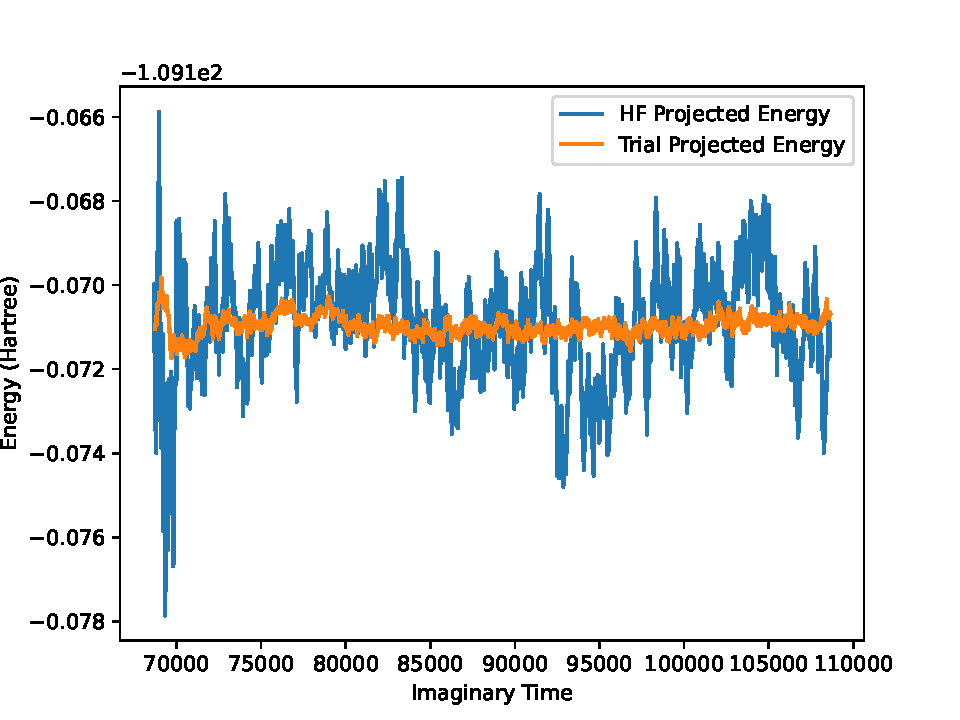
\includegraphics[width=0.8\textwidth]{figures/binding/trial_v_projE.pdf}
    \caption{The HF-projected and trial-projected energy trajectories in imaginary time for N$_2$ with a separation of $10$ Bohr with the \avtz basis set and the Jastrow factor optimised for the variance of the FCIQMC energy. The calculation was done with $10^8$ FCIQMC walkers. This is a highly dissociated and hence multireference state. The trial-projected energy uses the top 10 determinants but substantially improves the rate of convergence when compared to the HF projected energy.}
    \label{fig:trial_projected_energy}
\end{figure}
We can see from this figure that using the trial-projected energy even with just a few determinants allows us to much more easily handle highly multireference problems. Thus, trial wave functions are used throughout the rest of this chapter.

\section{Results}
\subsection{Computational Details}

We calculate the energy of the nitrogen molecule across multiple bond lengths, ranging from $1.92$ to $10$ Bohr. We use the \avtz basis set, which contains diffuse functions for long-range correlations while still being a modest size. We calculate the non-TC CI vectors and \glspl{1RDM} for each geometry with FCIQMC (using \neci),\supercite{gutherNECI2020} CASSCF (using \molpro),\supercite{wernerMOLPRO,wernerMolpro2012,wernerMolproQuantumChemistry2020} and CASCI (using \pyscf).\supercite{sunPySCF2018} The CI vector is then used in the objective function for optimising the Jastrow factor with VMC using \casino.\supercite{needsVariational2020} Using the optimised Jastrow factor and 1RDM, we then calculate the relevant integrals for the xTC Hamiltonian using \pytchint. Finally, xTC-FCIQMC is performed on these integrals with \neci. Each geometry is calculated independently; that is, the Jastrow factor is optimised for each geometry separately. In order to keep memory usage manageable, we cutoff the number of determinants in our CI vector to be $100$. Even at the dissociated limit, the number of relatively-highly-weighted determinants is around $20$, so $100$ should be enough to capture the static correlation for the VMC optimisation.

Next, we also calculate the vertical excited-state energies using this workflow for a few states of the nitrogen molecules with CASSCF- and CASCI-Jastrows. Excited states are also challenging multireference problems. Moreover, we optimise the Jastrow factors in a state-specific manner. That is, for some excited state $\Phi_\mathrm{exc}$, our ansatz becomes $\Psi_\mathrm{exc} = \e^J\Phi_\mathrm{exc}$, thereby modifying our workflow slightly to optimise specifically for that state, as well as using its 1RDM for the xTC approximation. Naturally, the xTC-FCIQMC calculation will be targeting this state. For cases where a triplet excited state of the same symmetry is lower in energy than a singlet excited state, the FCIQMC calculation will collapse to the triplet state. To overcome this, we use a spin-penalty term to target the singlet excited state.\supercite{weserSpin2022}

For the N$_2$ binding curve, we compare against the highly accurate experimental curve determined in reference \citenum{leroyAccurate2006}, and as a benchmark we compare against F12 calculations, performed in \molpro.\supercite{wernerMOLPRO,wernerMolpro2012,wernerMolproQuantumChemistry2020} For excited states we compare against extrapolated FCI calculations reported in reference \citenum{loosMountaineering2018}.

\subsection{Binding Curves}

As illustrated in figure \ref{fig:binding-curves-full-diss}, we obtain a qualitatively-correct binding curve for the nitrogen molecule using any of the Jastrow factors, besides the RHF-Jastrow. Shown in that figure is also a zoom-in on the dissociated limit, indicating the RHF-Jastrow curve is the only one exhibiting the pathological ``dip'' behaviour. The remaining unphysical behaviour amounts to noise, which has a few potential sources:
\begin{itemize}
    \item The optimisation of the Jastrow factor is done with VMC, a stochastic algorithm. As described in \autoref{chap:opt}, VMC optimisation for the TC method is complex, and as of yet has not been done on strongly multireference problems. Since the optimisation is done independently for each point along the binding curve, this may lead to some noise.
    \item The FCIQMC calculations are also stochastic, and this may also lead to some noise, particularly in the dissociated limit when not using a multideterminantal trial wave function.
    \item In the case of the FCIQMC-Jastrow, even the non-TC calculation prior to Jastrow optimisation is stochastic. In this case, the CI vector and 1RDM collected from the non-TC-FCIQMC calculation is done so at only a snapshot in imaginary time: right at the end of the calculation. One way to reduce this noise (not explored here) would be to average these values over imaginary time.
\end{itemize}
Thus, we can conclude that the biggest problem with the TC workflow has been resolved in three ways by introducing a multireference Jastrow optimisation (and 1RDM for the xTC approximation).

\begin{figure}[htbp]
    \centering
    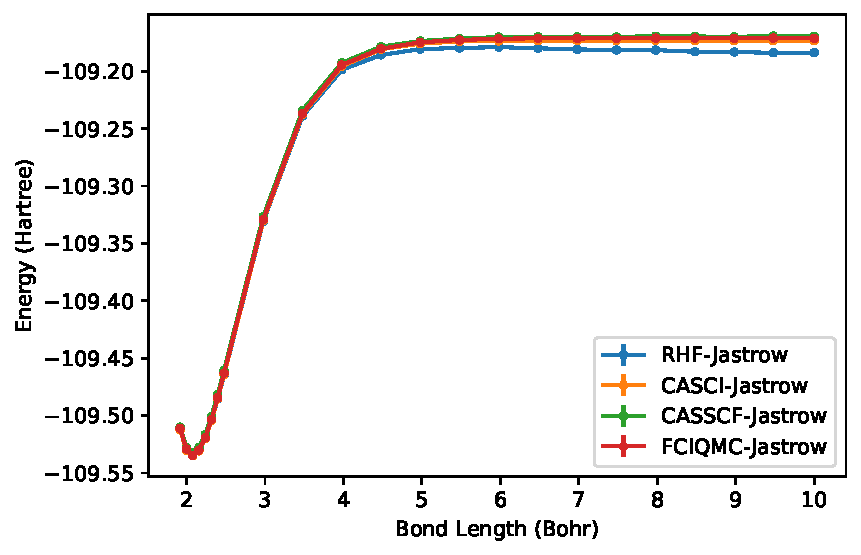
\includegraphics[width=0.8\textwidth]{figures/binding/all_binding_curves}
    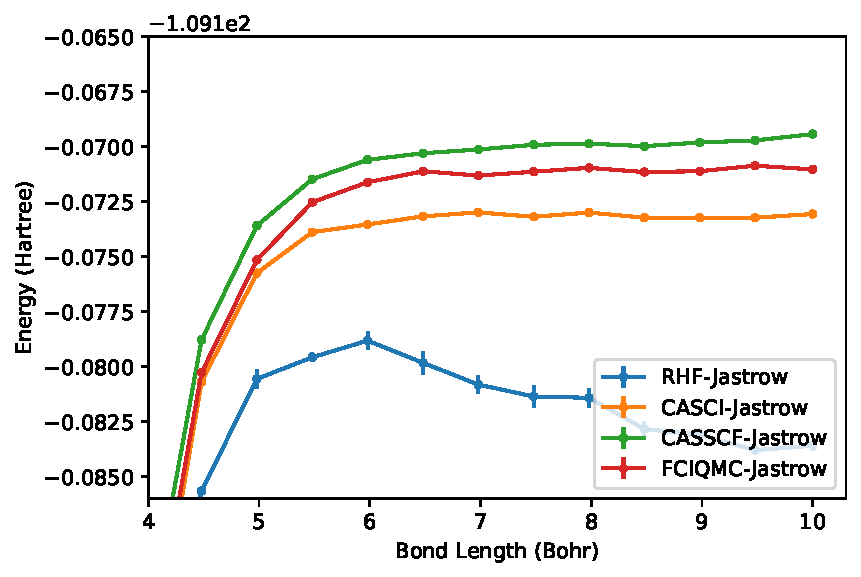
\includegraphics[width=0.8\textwidth]{figures/binding/all_binding_curves_dissociated}
    \caption{xTC-FCIQMC energies for the nitrogen dimer for various points along its binding curve, between 1.92 and 10 Bohr radii. Calculations were performed with the \avtz basis set. Four choices for Jastrow factors are presented. The forms for the actual Jastrow factor $J$ is the same, but the value for $\ket{\Phi}$ in the ansatz $\ket\Psi=\e^J\ket\Phi$ is different. The choices are: RHF-Jastrow (blue), CASCI-Jastrow (orange), CASSCF-Jastrow (green) and the FCIQMC-Jastrow (red). The top panel shows the full binding curve, while the bottom panel shows the dissociated limit. Notice that except for the RHF-Jastrow curve, these Jastrow factors result in qualitatively-correct xTC-FCIQMC binding curves. Noise near dissociation is likely due to the VMC optimisation, which was shown in \autoref{chap:opt} to have an error in the final TC energy of about 0.1 mHa.
    }
    \label{fig:binding-curves-full-diss}
\end{figure}

We now consider the binding curve at the equilibrium geometry (taken to be $2.08$ Bohr radii). Such a zoom-in is shown in figure \ref{fig:binding-curves-minimum}. Since N$_2$ is largely single-reference in this region, we expect all of the curves, including that with the RHF-Jastrow, to approximately be equal there. Relative to the RHF-Jastrow curve,
\begin{itemize}
    \item The CASCI-Jastrow curve uses the same orbitals and uses only a small subspace of the full CI space, and is indeed strongly single-reference in this region. As a result, this curve is almost identical to the RHF-Jastrow curve in the region around the minimum.
    \item The CASSCF-Jastrow curve has a noticeable shift of about $2.8$ mHa. While not expected, since the TC method is nonvariational we cannot guarantee a more complete wave function description to necessarily lead to a lower energy value. However, notice in the bottom panel of figure \ref{fig:binding-curves-full-diss} the CASSCF-Jastrow curve is shifted upwards relative to the CASCI-Jastrow curve by about the same amount, so in relative terms this is actually acceptable.
    \item The FCIQMC-Jastrow is slightly higher in energy compared to the RHF- and CASCI-Jastrow curves near the minimum, and similarly above the CASCI-Jastrow curve at dissociation. Since it shares the same orbitals as the CASCI-Jastrow curve, and we are primarily concerned with static correlation at this part of the workflow, we expect the FCIQMC-Jastrow curve to have a similar shape, and indeed it does. Possible sources of differences are: stochastic noise and having more flexibility to capture the full wave function (especially relevant at dissociation).
\end{itemize}

\begin{figure}[htbp]
    \centering
    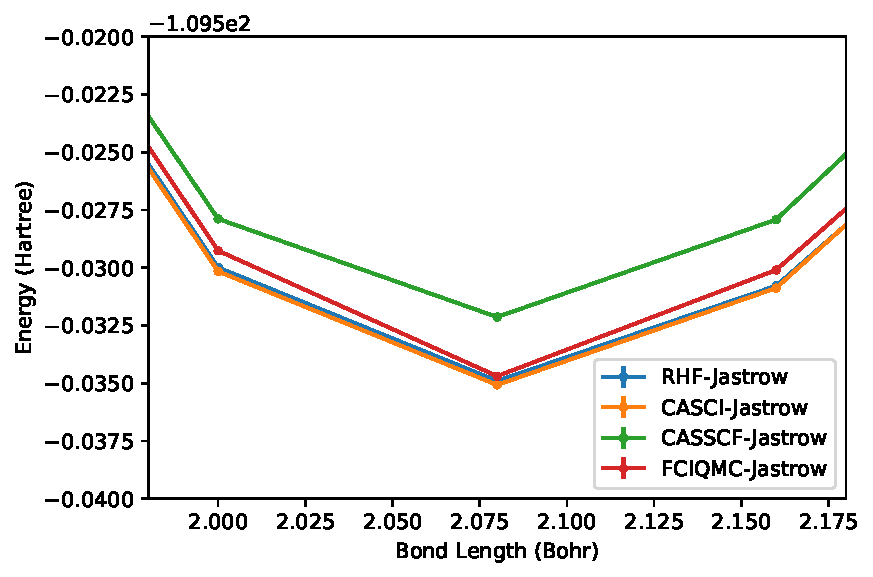
\includegraphics[width=0.8\textwidth]{figures/binding/all_binding_curves_min}
    \caption{The N$_2$ binding curves at \avtz for the RHF- (blue), CASCI- (orange), CASSCF- (green) and FCIQMC-Jastrow (red), zoomed in near equilibrium. Here, the problem is strongly single-reference and hence we expect all curves to be similar. However, the CASSCF-Jastrow curve is shifted upwards relative to the CASCI-Jastrow curve by about $2.8$ mHa, but this is compensated for at dissociation.}
    \label{fig:binding-curves-minimum}
\end{figure}

Naturally, we also wish to determine how accurate our calculations are. This is easy to verify for the extremes, as we can directly compare against \gls{HEAT}.\supercite{fellerSurvey2008} However, we also want to evaluate the accuracy of the rest of the binding curve. For this, we test against an accurate fit to experimental spectroscopic data which includes high-energy dissociated data.\supercite{leroyAccurate2006} Since we are only interested in relative energies, we normalise all curves to be zero at $10$ Bohr radii, and subtract the experimental values. The result of this is shown in figure \ref{fig:binding-curves-experiment}.

\begin{figure}[htbp]
    \centering
    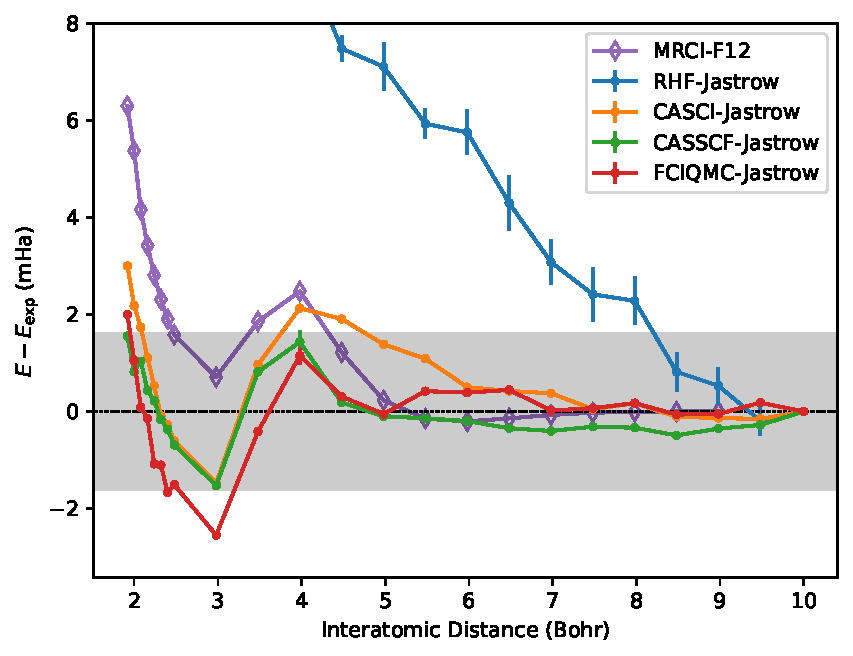
\includegraphics[width=0.8\textwidth]{figures/binding/residuals}
    \caption{Binding curves for each Jastrow factor optimisation strategy relative to the experimental fit from reference \citenum{leroyAccurate2006}. All curves are normalised such that the energy at $10$ Bohr radii is zero, except for MRCI-D-F12 where energy is set to zero at $8.98$ Bohr radii (past this, it did not converge). The shaded region represents $1.6$ mHa, so-called ``chemical accuracy''. We see that most of the curves for the multirefence Jastrow optimisations are within chemical accuracy, outperforming MRCI-D-F12. Note that while the relative values are below experiment for some regions (notably around $3$ Bohr), all absolute values are above the HEAT result for N$_2$ at equilibrium.}
    \label{fig:binding-curves-experiment}
\end{figure}

We find that the CASCI- and FCIQMC-Jastrow curves are within chemical accuracy (1.6 mHa) for most of the binding curve and the CASSCF-Jastrow entirely within chemical accuracy when compared against experiment, all of them outperforming MRCI-D-F12. It is worth noting, however, that unlike MRCI-D-F12, our multireference Jastrow factors are not uniformly above experiment. As expected, the RHF-Jastrow performs poorly.

Another worthwhile check is how accurate the atomisation energy is, taking the extremely dissociated limit ($10$ Bohr radii) and comparing it against equilibrium ($2.08$ Bohr radii). This is shown in table \ref{tbl:binding-atomisation-energies}. Relative to experiment, all multideterminantal Jastrow factors are within chemical accuracy ($1.6$ mHa).

\begin{table}[htbp]
    \centering
        \begin{tabular}{c|c}
            Jastrow Factor & Atomisation Energy (mHa) \\
            \hline
            CASCI & 362.0 \\
            CASSCF & 362.7 \\
            FCIQMC & 363.6 \\
            \bottomrule
            MRCI-D-F12 & 359.5 \\
            HEAT\supercite{fellerSurvey2008} & 363.9 \\
            Experiment\supercite{leroyAccurate2006} & 363.7
        \end{tabular}
    \caption{Atomisation energies using the binding curves for the multideterminantal Jastrow factor optimisation choices. Relative to experiment, all TC calculations are within chemical accuracy (1.6 mHa), with the CASI-Jastrow narrowly outside it relative to HEAT. The RHF-Jastrow is not included in the table because it does not stabilise to a dissociated limit. Note also that these values have an additional error coming from VMC of about $0.3$ mHa, according to the study from \autoref{chap:opt} ($0.1$ mHa error for the molecule, and for each atom). All multideterminantal Jastrow factors outperform MRCI-D-F12 according to this measure.}
    \label{tbl:binding-atomisation-energies}
\end{table}

Finally, as a measure for the size consistency error, we consider the difference between twice the atom's energy and that of the molecule at a separation of $10$ Bohr radii. This is shown in table \ref{tbl:size-consistency}. We find that the CASSCF- and FCIQMC-Jastrow factors are size consistent to a reasonable degree (similar to MRCI-D-F12) whereas the CASCI-Jastrow factor is not as size consistent. Non-TC CASCI was already size inconsistent, and the Jastrow optimisation was likely not able to adequately compensate for the missing dynamical correlation.

\begin{table}[htbp]
    \centering
    \begin{tabular}{c|c}
        Jastrow Factor & $\sum E_\mathrm{atom} - E_\mathrm{molecule}(r=10)$ (mHa) \\
        \hline
        CASCI & 2.1 \\
        CASSCF & -1.5 \\
        FCIQMC & 0.5 \\
        \bottomrule
        % Non-TC & -3.9(1) \\
        MRCI-D-F12 & -0.9
    \end{tabular}
    \caption{Size consistency error for the multideterminantal Jastrow optimisation choices, expressed as the difference between twice the energy of the atom and the energy of the molecule at dissociation. CASSCF- and FCIQMC-Jastrow factors show size consistency similar to MRCI-D-F12, which we use as a benchmark. The CASCI-Jastrow is has a larger error, but this is likely because the non-TC CASCI was already size inconsistent, and the Jastrow optimisation was not able to adequately compensate for the missing dynamical correlation. Including the RHF-Jastrow factor is meaningless because it does not stabilise in the dissociated limit.
    }
    \label{tbl:size-consistency}
\end{table}


\subsection{Excitation Energies}

One major advantage to this updated workflow is the ability to explicitly target specific states. We demonstrate this by calculating select excitation energies of the nitrogen molecule. We use two approaches to generate the Jastrow factors $J$, both based on the full valence $(10o,8e)$ active space:
\begin{itemize}
    \item CASCI$(10o,8e)$-$J$, where the CI vector is chosen ``minimally''; that is, we take 99\% of the total wave function as measured by the squared modulus of the coefficients (and including additional determinants if degenerate). This, for example, results in only the RHF determinant in the ground state, and only two in the excited states, plus possibly some very small additional determinants being included in the CI vector. This approach does no additional optimisation of the orbitals beyond RHF.
    \item \Gls{SA}-CASSCF$(10o,8e)$-$J$, where all states are included in the orbital optimisation (therefore, all states share the same orbitals). For each state, we use the top $100$ determinants of the CI vector as the $\Phi$ ansatz.
\end{itemize}
The CASCI or CASSCF calculations are used to then determine the 1RDM for the state. The CI vector is then used in the VMC optimisation, and the 1RDM for the xTC approximation when calculating integrals. For simplicity, we consider only those states which are the lowest in their symmetry, which allows us to use standard ground-state FCIQMC for the excited states.\footnote{In principle, we may also target higher-order excited states, but this would require an additional adjoint replica.\supercite{bluntExcitedstateApproachFull2015}}

% For the CASSCF calculations, we try both state-specific CASSCF as well as \gls{SA}-CASSCF.


\begin{figure}[htbp]
    \centering
    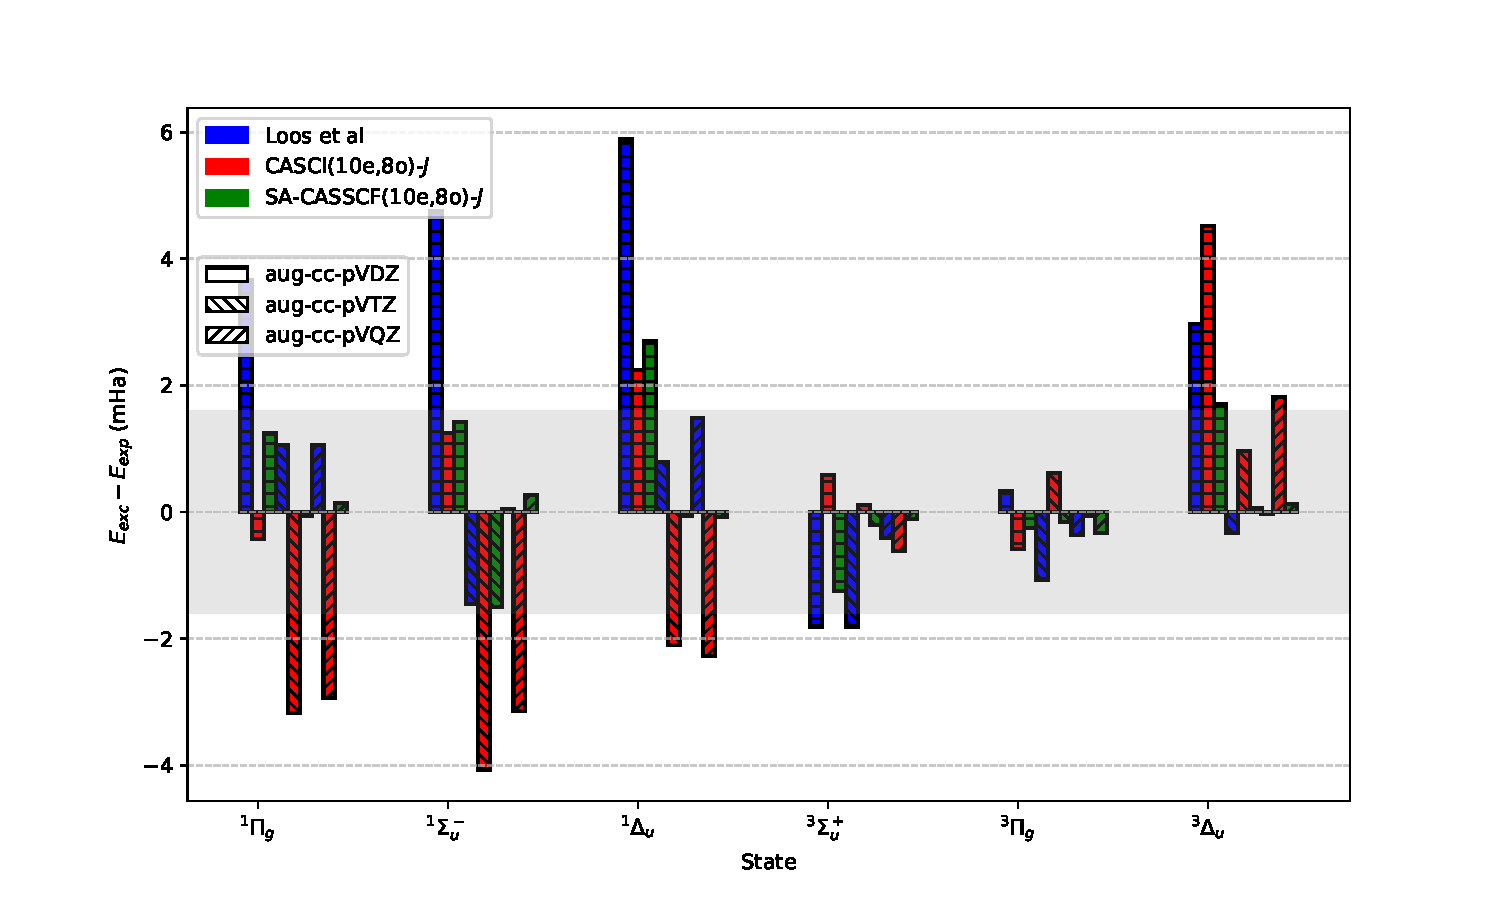
\includegraphics[width=\textwidth]{figures/binding/n2_exc}
    \caption{Excitation energies $E_\mathrm{exc}$ for each state compared to experiment $E_\mathrm{exp}$,\supercite{oddershedeComparison1985,huberConstants1979} $E_\mathrm{exc}-E_\mathrm{exp}$ for the nitrogen dimer. Shown are the results from extrapolated FCI (exFCI), taken from reference \citenum{loosMountaineering2018}, xTC-FCIQMC with CASCI-Jastrow factors and xTC-FCIQMC with state-averaged CASSCF-Jastrow factors for the \avdz (horizontal stripes), \avtz (backslash hatch pattern) and \avqz (forward-slash hatch pattern) basis sets. The SA-CASSCF Jastrow factors are shown to largely outperform the other two approaches, being generally within chemical accuracy, even for relatively modest basis sets. The CASCI Jastrow factors perform unfavourably, however. This could be because the orbitals are not optimised for the active space, or it could be because the CI vector is shorter, and the number of determinants for each state is not consistent. Therefore, it is reasonable to assert that the use of the transcorrelated method with optimised orbitals and tailored Jastrow factors allow for highly accurate excitation energies.
        }
    \label{fig:n2-excite-relative}
\end{figure}

Figure \ref{fig:n2-excite-relative} displays the excitation energies $E_\mathrm{exc}$ of the N$_2$. Of the three methods explored (xTC-FCIQMC with SA-CASSCF- or CASCI-Jastrow factors, and non-TC), SA-CASSCF-Jastrow factors give the most consistently accurate excitation energies. The SA-CASSCF-Jastrow factors result in excitation energies typically within chemical accuracy even with \avdz, and consistently in chemical accuracy for \avtz and \avqz. This suggests a SA-CASSCF is a particularly fruitful ansatz for $\Phi$ when used in the TC method to calculate excited states.

\begin{table}[htbp]
\centering
\begin{threeparttable}
\begin{tabular}{c|cccc||c}
\multicolumn{6}{c}{\textbf{Dinitrogen}} \\
State & Method & \avdz & \avtz & \avqz & Benchmarks \\
\hline
\multirow{3}{*}{$^1\Pi_g$}
& non-TC exFCI\tnote{a} & 345.8  & 343.2 & 343.2 & 344.47\tnote{b} \\
& CASCI-xTC    & 341.7 & 339.0 & 339.2 & 344.47\tnote{c}  \\
& SA-CASSCF-xTC   & 343.4 & 342.1 & 342.3 & 342.99\tnote{d}  \\
\hline
\multirow{3}{*}{$^1\Sigma_u^-$}
& non-TC exFCI\tnote{a}       & 369.3 & 363.1 & 364.6  & 367.04\tnote{b} \\
& CASCI-xTC          & 365.8 & 360.5 & 361.4   & 367.04\tnote{c}  \\
& SA-CASSCF-xTC         & 366.0 & 363.1 & 364.8   & 373.33\tnote{d}  \\
\hline
\multirow{3}{*}{$^1\Delta_u$}
& non-TC exFCI\tnote{a}       & 383.3 & 378.2 & 378.9 & 379.99\tnote{b} \\
& CASCI-xTC          & 379.7 & 375.3 & 375.1  & 379.99\tnote{c}  \\
& SA-CASSCF-xTC         & 380.1 & 377.3 & 377.3   & 389.98\tnote{d}  \\
\hline
\multirow{3}{*}{$^3\Sigma_u^+$}
& non-TC exFCI\tnote{a}       & 283.0 & 283.0 & 284.4  & 286.75\tnote{b} \\
& CASCI-xTC          & 285.4 & 284.9 & 284.2  & 286.75\tnote{c}  \\
& SA-CASSCF-xTC         & 283.6 & 284.6 & 284.7 & 279.72\tnote{d}  \\
\hline
\multirow{3}{*}{$^3\Pi_g$}
& non-TC exFCI\tnote{a}       & 295.8 &  294.4& 295.1  & 297.48\tnote{b} \\
& CASCI-xTC          & 294.9 & 296.1 & 295.4  & 297.48\tnote{c}  \\
& SA-CASSCF-xTC         & 295.2 & 295.3 & 295.1 & 297.85\tnote{d}  \\
\hline
\multirow{3}{*}{$^3\Delta_u$}
& non-TC exFCI\tnote{a}       & 329.3 &  326.0 & 326.3   & 328.56\tnote{b} \\
& CASCI-xTC          & 330.8 & 327.3 & 328.2   & 328.56\tnote{c}  \\
& SA-CASSCF-xTC         & 328.0 & 326.4 & 326.5 & 330.41\tnote{d}  \\
\bottomrule
\end{tabular}
\begin{tablenotes}
    \item[a] Taken from reference \citenum{loosMountaineering2018}.
    \item[b] Experimental value, see references \parencite{loosMountaineering2018,oddershedeComparison1985,huberConstants1979} .
    \item[c] Experimental value, see references \parencite{loosMountaineering2018,nielsenTransition1980,huberConstants1979}.
    \item[d] Theoretical (multireference coupled cluster) value, see references \parencite{loosMountaineering2018,ben-shlomoN21990}.
\end{tablenotes}
\end{threeparttable}
\caption{
    Excitation energies for the nitrogen dimer various excited states, in mHa. We use xTC-FCIQMC with CASCI- or SA-CASSCF orbitals and CI vector ansatz for the TC method, and compare it to experiment and non-TC results. We find that while no method consistently beats all others, SA-CASSCF is a particularly effective choice for calculating excited states in the context of TC.
    }
\label{tbl:excitation-energies-n2}
\end{table}

The excitation energies are presented in tabular format in table \ref{tbl:excitation-energies-n2}. Here we can see again the relative efficacy of SA-CASSCF orbitals and CI vectors for use for the TC method, compared to experimental values.

\subsubsection{CAS-Only TC Excitation Energies}

Since CASSCF primarily serves to capture the effects of \emph{static} correlation, whereas TC is designed to capture the effects of \emph{dynamical} correlation, it is interesting to see how well the method performs when we perform our calculations only inside the active space. For this, we use the SA-CASSCF$(10e,8o)$-Jastrow factors from before, but instead of performing all-electron xTC-FCIQMC, we instead only diagonalise the Hamiltonian in the active space. That is, we perform a xTC-CASCI$(10e,8o)$ calculation, using the orbitals optimised by the non-TC SA-CASSCF calculation. The xTC-CASCI calculations were performed using \neci.\supercite{gutherNECI2020}

\begin{figure}[htbp]
    \centering
    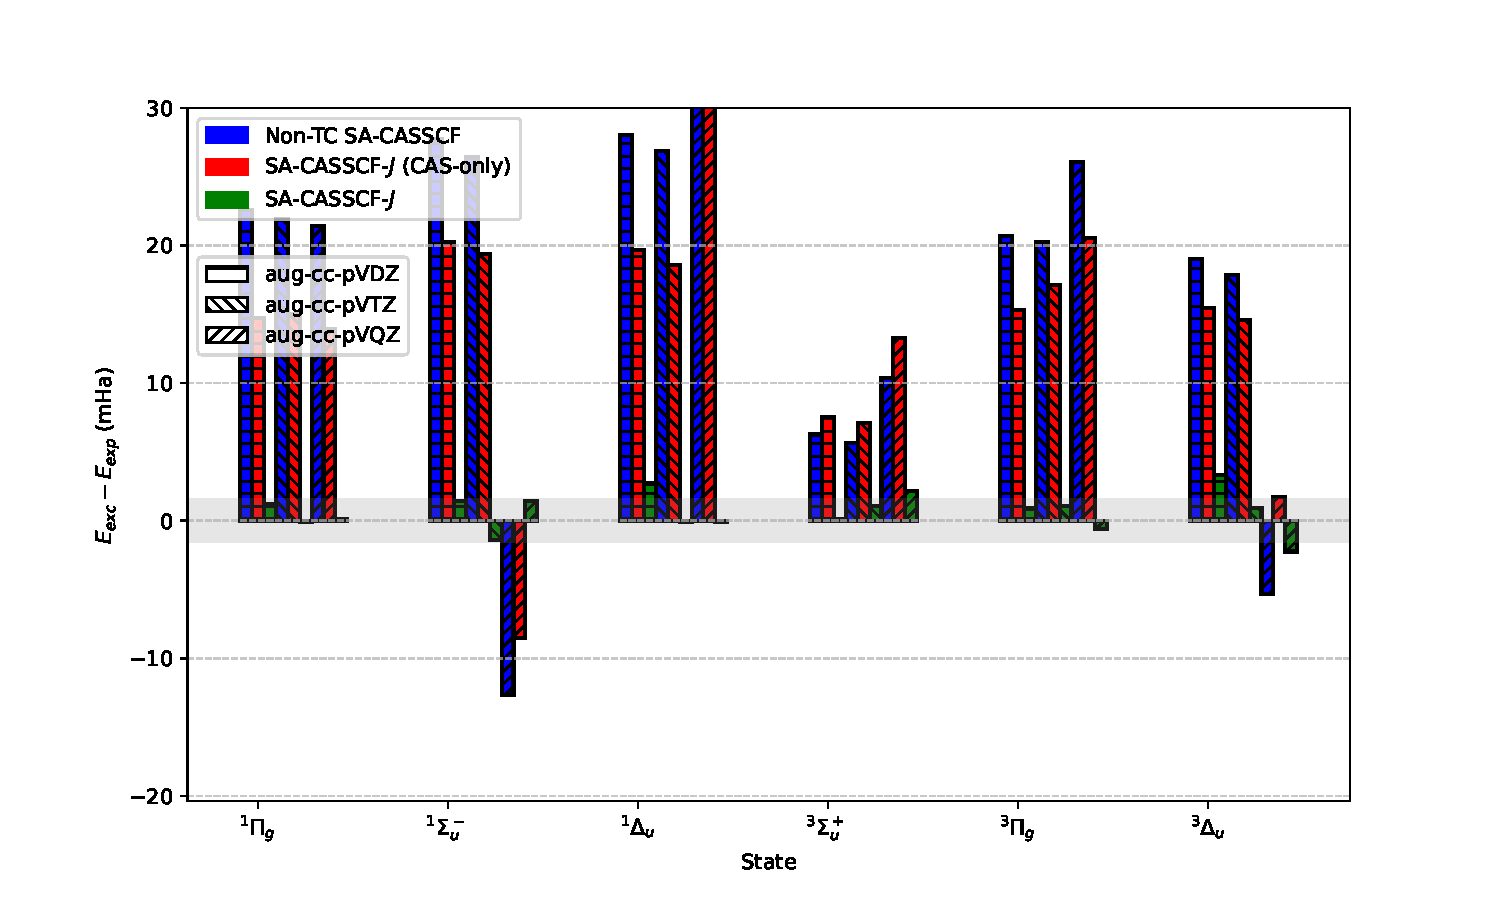
\includegraphics[width=\textwidth]{figures/binding/n2_exc_cas.pdf}
    \caption{Excitation energies relative to experiment for a few states of N$_2$. For comparison, we show using non-TC SA-CASSCF, as well as xTC-FCIQMC (all electrons and all virtual orbitals included) and xTC-CASCI$(10e,8o)$ using the SA-CASSCF-Jastrow factor. As expected, the non-TC SA-CASSCF is not able to sufficiently capture all correlation effects of the excited states, resulting in highly overestimated excitation energies.
    The xTC CAS-only calculations improve on these, suggesting that the Jastrow factor is able to differentially capture some of the dynamical correlation missing in the SA-CASSCF calculation. However, since the resulting excitation energies are still largely outside chemical accuracy, some additional correlation via virtual orbitals needs to be included to achieve chemical accuracy.
    % The xTC CAS-only calculations improve on these, but are still largely outside chemical accuracy, and still far from all-electron FCIQMC with all virtuals included in the correlation calculation. This suggests that some of the dynamical correlation missing in the SA-CASSCF calculation is captured by the Jastrow factor.
    }
    \label{fig:n2-excite-relative-cas}
\end{figure}

Results are shown in figure \ref{fig:n2-excite-relative-cas}. As shown, non-TC SA-CASSCF fails to capture all correlation effects of the excited states and tends to overestimate the excitation energies. The xTC CAS-only calculations are better, although still far from desired accuracy, and not nearly as accurate as the all-electron xTC calculations. However, since the diagonalisation is performed only in a small active space, this is still a noteworthy improvement.


\section{Conclusion and Outlook}

We have presented a framework for using the transcorrelated method for solving problems of strongly multireference character. We find challenging problems like the nitrogen dissociation curve may be solved by modifying the ansatz for $\Phi$ with a multireference CI expansion, and appropriately changing the corresponding 1RDM for use in the xTC approximation. Particularly effective choices for $\Phi$ are FCIQMC and CASSCF. Using a small FCIQMC calculation has already been found to effectively solve the issues experienced with a HF ansatz, and its use with \glspl{ECP} to efficienctly describe the core region with TC has already been explored.\supercite{simulaEcp}

Furthermore, with this methodology we can tailor our TC Hamiltonian to target specific states of interest. Using state-averaged CASSCF, we find that this approach yields accurate results for excitation energies of the nitrogen dimer. Moreoever, we show that by combining the TC method to capture dynamical correlation with CASSCF to capture static correlation, we have improved accuracy. However, results suggest we may need larger active spaces and/or a transcorrelated perturbative treatment such as xTC-\gls{CASPT2}.

While this approach has already proven remarkably effective for a few systems, one key outlook is to study a wider array of complex problems, including transition metals and periodic solids, in addition to a larger selection of smaller molecules beyond N$_2$. We may also wish to continue the procedure self-consistently. That is, we may use the resulting right-eigenvector of $\htc$ as the ansatz for $\Phi$ in a subsequent calculation (as well as use the 1RDM, which may now be non-Hermitian), and continue until some convergence is achieved. Similarly, this study is a promising start for a \gls{TC}-\gls{MCSCF} method, wherein the orbitals, CI coefficients, and Jastrow factor parameters are all optimised simultaneously with a self-consistent algorithm, and no all-electron TC calculation is required or, as mentioned, we might add a transcorrelated perturbative correction as in \gls{CASPT2}.
